\section{Resultados}
%###########################
%########## AVG ############
\subsection{Dinámicas factorizables}
\begin{frame}{Dinámicas factorizables}
    Por dinámicas factorizables entendemos\pause:
    \begin{equation}
        \mcH=\sum_{k=1}^{n}\omega_{k}\Id_{2^{k-1}}\otimes H_{k} \otimes \Id_{2^{n-k}},\nonumber
    \end{equation}
    Las unitarias:\pause
    \begin{equation}
        \mcU_{t}=\Motimes_{k=1}^{n}\text{exp}\qty(-\rmi\omega_{k}H_{k}t)=\Motimes_{k=1}^{n} U_{k}(t).\nonumber
    \end{equation}\pause
    \begin{columns}
        \begin{column}{0.5\textwidth}
            El estado de máxima entropía es\pause
            \begin{equation}
                \varrho_{\max}(t)=\Motimes_{k=1}^{n}{\color{blue}\frac{1}{Z_{k}}}U_{k}(t) {\color{blue}e^{\qty(p_{k}\sum_{j}\lambda_{j}\pauli{j})}} (U_{k}(t))^{\dag}\nonumber
            \end{equation}
        \end{column}
        \pause
        \begin{column}{0.5\textwidth}
            La dinámica efectiva tiene expresión general\pause
            \begin{equation}
                \Gamma_{t}(\rho_{\ef})=\sum_{k=1}^{n}p_{k} U_{k}(t) {\color{blue}\rho_{k}} (U_{k}(t))^{\dag}.\nonumber
            \end{equation}
        \end{column}
    \end{columns}
\end{frame}
\begin{frame}{Partículas no interactuantes con diferente frecuencia de transición}
    \begin{columns}
        \begin{column}{0.5\textwidth}
            Usamos el hamiltoniano $\mcH=\sum_{k=1}^{n}\omega_{k}\pauli{3,k}$.\\ \pause
            Los valores $\expval{\pauli{k}(t)}_{\ef}\equiv\Tr(\pauli{k}\Gamma_{t}(\rho_{\ef}))$:\pause
            \begin{equation}
                \begin{gathered}
                \expval{\pauli{1}(t)}_{\ef}=p_{1} \expval{\sigma_{1}(t)}_{1}+\sum_{k=2}^{n}p_{k}\expval{\pauli{1}(t)}_{k}\text{\footnotemark}\pause\\
                \expval{\pauli{2}(t)}_{\ef}=p_{1} \expval{\sigma_{2}(t)}_{1}+\sum_{k=2}^{n}p_{k}\expval{\pauli{2}(t)}_{k}\pause\\
                \expval{\pauli{3}(t)}_{\ef}=\expval{\pauli{3}(0)}_{\ef}.
            \end{gathered}\nonumber
        \end{equation}
        \footnotetext{$^{1}$Aquí, $\expval{\pauli{1}(t)}_{k}=\Tr[\pauli{1}e^{-\rmi\omega_{k} t\pauli{3}} \rho_{k} e^{\rmi\omega_{k} t\pauli{3}}]$}
        \end{column}
        \pause
        \begin{column}{0.5\textwidth}
            Sea $p_{j\neq 1}=p_{\text{np}}=\frac{1-p_{1}}{1-n}$ y $r_{3,\ef}=0$.\pause\\
            Las expresiones se reducen a:\pause
            \begin{equation}
                \begin{gathered}
                    r_{1,\ef}(t)=p_{1}r_{1,1}(t)-p_{\text{np}}r_{\text{np}}\sum_{k=2}^{n}\sin(2\omega_{k} t-\phi)\pause\\
                    r_{2,\ef}(t)=p_{1}r_{2,1}(t)+p_{\text{np}}r_{\text{np}}\sum_{k=2}^{n}\sin(2\omega_{k} t+\theta).
                \end{gathered}\nonumber
            \end{equation}\pause
            donde\pause
            \begin{equation}
                r_{\text{np}}=\tanh(p_{\text{np}} \lambda).\nonumber
            \end{equation}
        \end{column}
    \end{columns}
\end{frame}
\begin{frame}{Convergencia}
    \begin{columns}
        \begin{column}{0.5\textwidth}
            Importante: límite $n\rightarrow\infty$. \pause
            \begin{equation}
                r_{1,\ef}(t)=p_{1}r_{1,1}(t)-p_{\text{np}}r_{\text{np}}\sum_{k=2}^{n}\sin(2\omega_{k} t-\phi)\nonumber
            \end{equation}\pause
            Sumas trigonométricas $\xrightarrow{n\rightarrow\infty} N(0,\text{std})$ \pause \\
            \vspace{0.3cm}
            La dinámica efectiva tiende a\pause  \\
\begin{equation}\label{eq:MeanDynamics}
    \Gamma_{t\rightarrow\infty}(\vec{r}_{\ef})\rightarrow\begin{pmatrix}
        p_{1}r_{1,1}(t)\\
        p_{1}r_{2,1}(t)\\
        r_{3}\\
    \end{pmatrix}\nonumber.
\end{equation}
        \end{column}
        \pause
        \begin{column}{0.5\textwidth}
           \begin{figure}
            \centering
            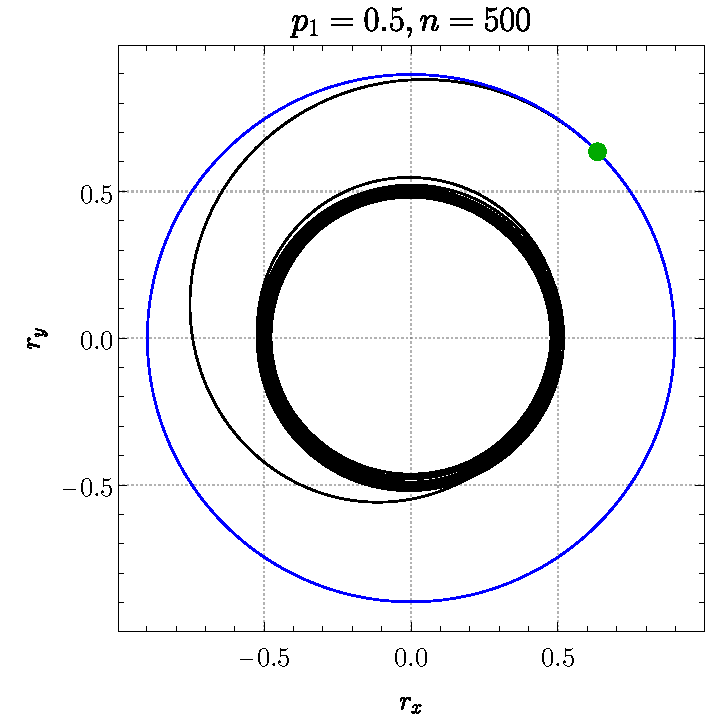
\includegraphics[width=1.\textwidth]{figures/maxent_results/local_all_ran_p=0.5_r=0.9_n=500_a=-3_b=3.pdf}
           \end{figure}
        \end{column}
    \end{columns}
\end{frame}
\begin{frame}{Convergencia}
    \begin{figure}
        \begin{subfigure}{0.45\textwidth}
            \centering
            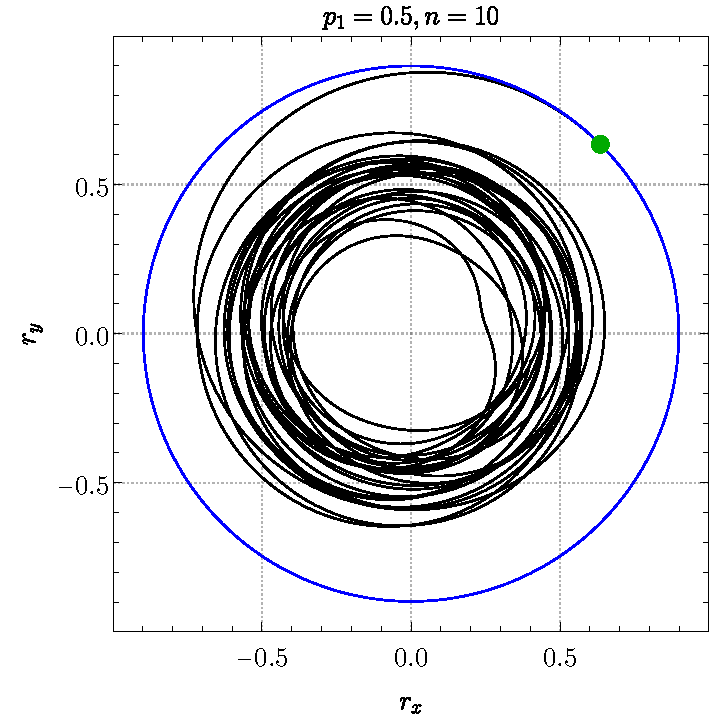
\includegraphics[width=1.\textwidth]{figures/maxent_results/local_all_ran_p=0.5_r=0.9_n=10_a=-3_b=3.pdf}
        \end{subfigure}
        \begin{subfigure}{0.45\textwidth}
            \centering
            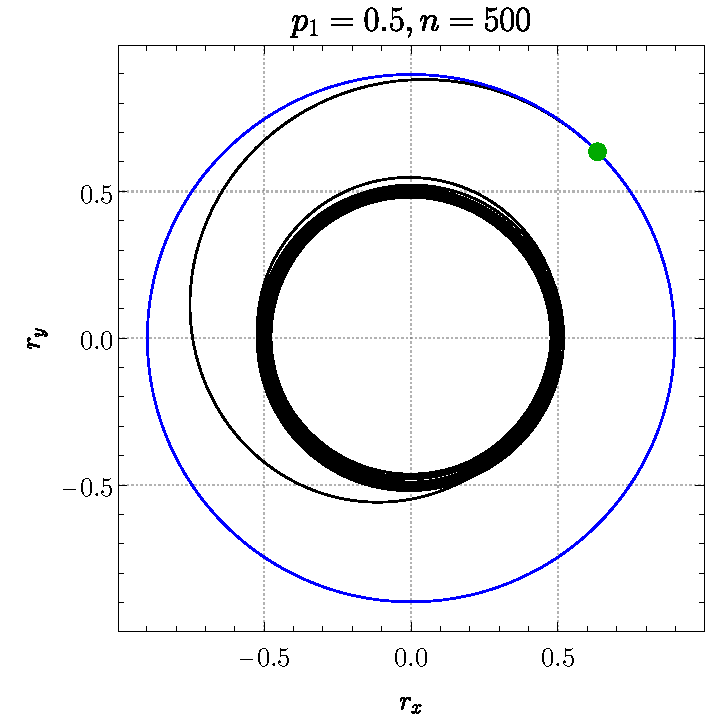
\includegraphics[width=1.\textwidth]{figures/maxent_results/local_all_ran_p=0.5_r=0.9_n=500_a=-3_b=3.pdf}
        \end{subfigure}
        \caption{CAPTION}
       \end{figure}
\end{frame}
%###########################


%###########################
%########## AVG ############
\subsection{Compuertas de cómputo cuántico}
\begin{frame}{Compuerta SWAP}
    \begin{columns}
        \begin{column}{0.5\textwidth}
            Estado efectivo antes y después:
            \begin{align*}
                \rho(0)&=p\rho_{A}+(1-p)\rho_{B},\\
                \rho(t=1)&=(1-p)\rho_{A}+p\rho_{B}.
                \end{align*}\pause
                Esto es una contracción:
                \begin{equation*}
                    \kappa_{t}=\frac{r_{\rho(1)}}{r_{\rho(0)}}.
                  \end{equation*}\pause
                  Canal de despolarización no lineal:\pause
                  \begin{center}
                    \tcbox{$\rho\mapsto\kappa_{1}^{\rho}\rho+(1-\kappa_{1}^{\rho})\frac{1}{2}\Id$}
                  \end{center}
        \end{column}\pause
        \begin{column}{0.5\textwidth}
            \begin{figure}[h!]
                \centering
                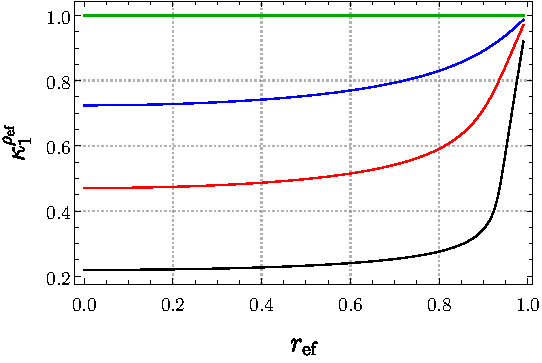
\includegraphics[width=0.9\linewidth]{figures/maxent_results/K(r).pdf}
                \caption{Depolarizing coefficient as a function of $r_{\rho(0)}$ for different values of $p$.}
              \end{figure}
        \end{column}
    \end{columns}
\end{frame}
\begin{frame}{Compuerta CNOT}
    \begin{columns}
        \begin{column}{0.5\textwidth}
            Estudiamos:
            \begin{equation}
                \rho(t=1)=\CG{\cnot \mcA_{\mcC}^{max}[\rho(0)](\cnot)^{\dag}}\nonumber
            \end{equation}
        \end{column}\pause
        \begin{column}{0.5\textwidth}
            El estado efectivo inicial es
            \begin{equation}
                \rho(0)=p\rho_{A}+(1-p)\rho_{B}.\nonumber
            \end{equation}
        \end{column}\pause
    \end{columns}
    El estado efectivo final es\pause
    \begin{align*}
        \rho(t=1)=&\frac{1}{2}\rho(0)\\
        &+\frac{(1-p)}{2}\qty[{\color{red}\expval{\pauli{1}}_{\rho_{B}}\rho_{A}+(1-\expval{\pauli{1}}_{\rho_{B}})\pauli{3}\rho_{A}\pauli{3}}]\\
        &+\frac{p}{2}\qty[{\color{blue}\expval{\pauli{3}}_{\rho_{A}}\rho_{B}+(1-\expval{\pauli{3}}_{\rho_{A}})\pauli{1}\rho_{B}\pauli{1}}].
    \end{align*}\pause
    Combinación de un canal no lineal de {\color{red}desfasamiento} y un canal no lineal de {\color{blue}bit flip}.
\end{frame}
\begin{frame}{Caso límite: canal de desfasamiento}
    \begin{columns}
        \begin{column}{0.5\textwidth}
            Supongamos $p=0$. El estado efectivo evolucionado:
            \begin{equation*}
              \rho(t=1)=\frac{1}{2}\rho(0)+\frac{1}{2}\pauli{3}\rho(0)\pauli{3}.
            \end{equation*}\pause
            ¡Esto es un canal de desfasamiento!\pause
        \end{column}
        \begin{column}{0.5\textwidth}
            \begin{figure}[h!]
                \centering
                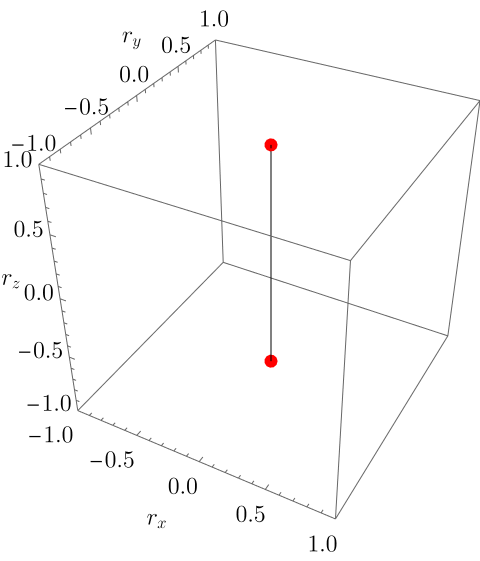
\includegraphics[width=0.7\linewidth]{figures/maxent_results/CNOT_p=1._t=1_r=0.9.png}
                \caption{Canal de desfasamiento}
              \end{figure}
        \end{column}
    \end{columns}
\end{frame}
\begin{frame}{Caso límite: canal de bitflip}
    \begin{columns}
        \begin{column}{0.5\textwidth}
            Supongamos $p=1$. El estado efectivo evolucionado:
            \begin{equation*}
              \rho(t=1)=\frac{1}{2}\rho(0)+\frac{1}{2}\pauli{1}\rho(0)\pauli{1}.
            \end{equation*}\pause
        
            ¡Esto es un canal de bit flip!\pause
        \end{column}
        \begin{column}{0.5\textwidth}
            \begin{figure}[h!]
                \centering
                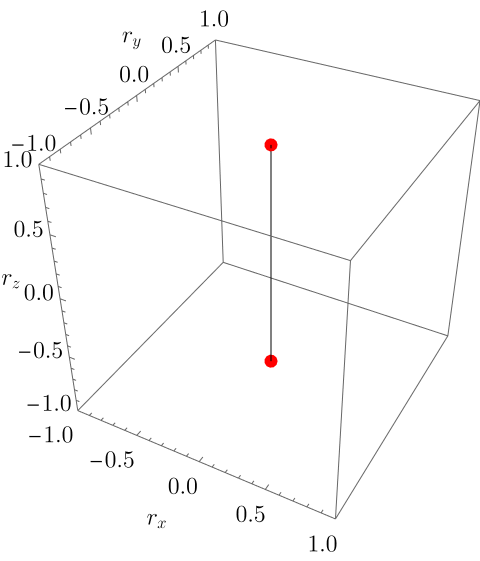
\includegraphics[width=0.7\linewidth]{figures/maxent_results/CNOT_p=1._t=1_r=0.9.png}
                \caption{Canal de bit flip}
                \label{fig:SWAPFactor2D}
              \end{figure}
        \end{column}
    \end{columns}
\end{frame}
\begin{frame}{CNOT efectivo sobre la esfera de Bloch}
    \begin{figure}[h!]
        \centering
        \begin{subfigure}{0.32\textwidth}
            \centering
            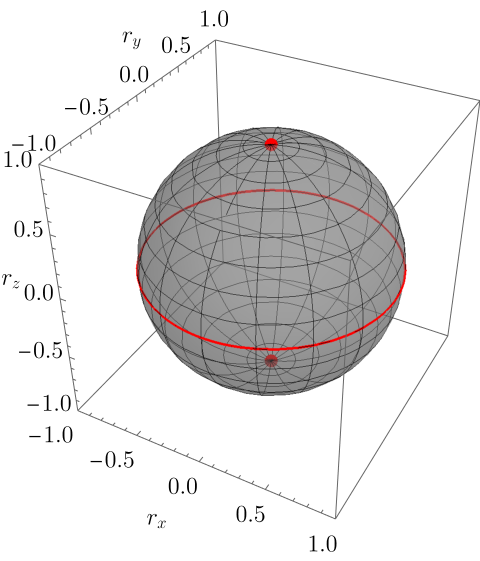
\includegraphics[width=0.9\linewidth]{figures/maxent_results/CNOT_p=0.5_t=0._r=0.9.png}
            \caption{$t=0.0$}
        \end{subfigure}%
        \begin{subfigure}{0.32\textwidth}
            \centering
            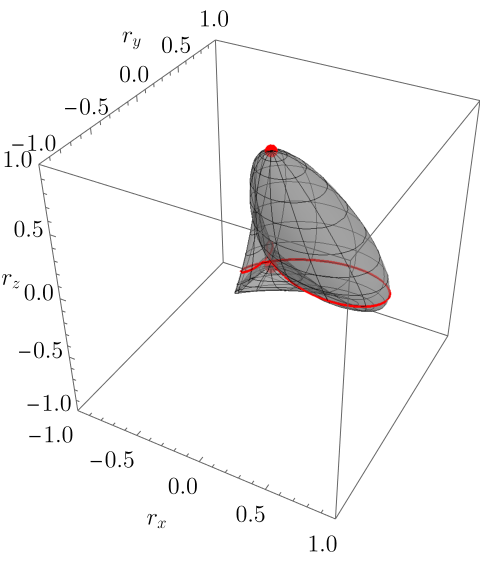
\includegraphics[width=0.9\linewidth]{figures/maxent_results/CNOT_p=0.5_t=1._r=0.9.png}
            \caption{$t=1.0$}
        \end{subfigure}
        \caption{Efecto sobre la esfera de Bloch. $r=0.8$, $p=0.4$.}
    \end{figure}
\end{frame}
%###########################


%###########################
%########## AVG ############
\subsection{Dinámicas especiales}

\begin{frame}{Canales de Pauli de N qubits}
    \begin{columns}
        \begin{column}{0.5\textwidth}
            Un canal de Pauli sobre un qubit,
            \begin{equation}
                \begin{gathered}
                P:\mcB(\hilbert_{2}) \rightarrow \mcB(\hilbert_{2})\nonumber\pause\\
                P(\Delta)=\sum_{k}q_{k}\pauli{k}\Delta\pauli{k} \rlap{,}
                \end{gathered}
            \end{equation}\pause
            aplica $\pauli{k}$ con probabilidad $q_{k}$.
        \end{column}
        \pause
        \begin{column}{0.5\textwidth}
            El canal de Pauli sobre $n$ qubits:
            \begin{equation}
                \begin{gathered}
                P:\mcB(\hilbert_{2^{n}}) \rightarrow \mcB(\hilbert_{2^{n}})\nonumber\pause\\
                P(\Delta)=\sum_{\vec{\alpha}}q_{\vec{\alpha}}\pauli{\vec{\alpha}}\Delta\pauli{\vec{\alpha}},\pause \,\text{ }\, \alpha_{k}\in\{0,1,2,3\} \rlap{.}
                \end{gathered}
            \end{equation}\pause
            donde  $\pauli{\vec{\alpha}}=\pauli{\alpha_{1}}\otimes\pauli{\alpha_{2}}\otimes...\otimes \pauli{\alpha_{n}}$.
        \end{column}
    \end{columns}
\end{frame}

\begin{frame}{Canales de desfasamiento y despolarización}
    \begin{columns}
        \begin{column}{0.5\textwidth}
            \begin{block}{Desfasamiento}
                El canal de Pauli
                \begin{equation}
                    P_{n,\pauli{j}}(\Delta)=\sum_{\vec{\alpha}}q_{\vec{\alpha}}\pauli{\vec{\alpha}}\Delta\pauli{\vec{\alpha}}, \,\text{ }\, \alpha_{k}\in\{0,j\}\nonumber
                \end{equation}\pause
                es  de desfasamiento si $q_{\vec{\alpha}\neq\vec{0}}=\frac{1-q_{\vec{0} }}{2^{n}-1}$\pause y 
                \begin{align}
                    \Gamma_{t}(\rho_{\ef})=&\qty(q_{\vec{0}}+\frac{2^{n-1}-1}{2^{n}-1}(1-q_{\vec{0}}))\rho_{\ef}\nonumber\\
                    &+\qty(\frac{2^{n-1}}{2^{n}-1}(1-q_{\vec{0}}))\pauli{j}\rho_{\ef}\pauli{j}.\nonumber
                \end{align}
            \end{block}
        \end{column}\pause
        \begin{column}{0.5\textwidth}
            \begin{block}{Despolarización}
                Para $n$ qubits:\pause
                \begin{equation}
                    \begin{gathered}
                    D_{q}:\mcB(\hilbert_{2^{n}}) \rightarrow \mcB(\hilbert_{2^{n}})\\
                    D_{q}(\Delta)=q\Delta+(1-q)\Id_{2^{n}}\Tr(\Delta)\rlap{.}
                \end{gathered}\nonumber
            \end{equation}\pause
                La dinámica efectiva que corresponde al canal de despolarización es\pause
                \begin{equation}
                    \Gamma_{t}(\rho_{\ef})=q\rho_{\ef}+(1-q)\Id_{2},\nonumber
                \end{equation}\pause
                ¡Otro canal de despolarización!
            \end{block}
        \end{column}
    \end{columns}
\end{frame}

\begin{frame}{Canal de estabilización}
    \begin{columns}
        \begin{column}{0.5\textwidth}
            El canal de estabilización.
            \begin{gather}
                \mcE_{\psi,t}:\mcB(\hilbert_{2^{n}}) \rightarrow \mcB(\hilbert_{2^{n}})\nonumber\pause\\
                \mcE_{\psi,t}(\Delta)=e^{-t\mu}\varrho+(1-e^{-t \mu})\dyad{\psi}\Tr(\Delta)\rlap{.}\nonumber\pause
            \end{gather}
            donde $\dyad{\psi}\in \densityspace{2^{n}}$
        \end{column}\pause
        \begin{column}{0.5\textwidth}
            La dinámica efectiva:\pause
            \begin{equation}\label{eq:EffectiveStabilizing}
                \Gamma_{t}(\rho_{\ef})=e^{-t\mu}\rho(0)+(1-e^{-t \mu})\mcC(\dyad{\psi}).\nonumber
            \end{equation}\pause
            Canal cuántico, pero no necesariamente un canal de estabilización: ¡puede ser despolarización!
        \end{column}
    \end{columns}
\end{frame}
%###########################


%###########################
%########## AVG ############
\subsection{La asignación promedio}
\begin{frame}{Construcción de la asignación promedio}
    Otra forma de escoger un estado microscópico compatible es tomando un promedio\mycite{Macro-To-Micro}. Un promedio sobre el conjunto
    \begin{equation}
        \Omega_{\mcC}(\rho_{\ef}) = \{\ket{\psi}\in\hilbert_{m}:\, \mcC(\dyad{\psi}) = \rho_{\ef}  \}.\nonumber
    \end{equation}
    La aplicación de asignación promedio es el promedio sobre dicho conjunto\mycite{priv}, \ie 
    \begin{equation}
        \mcA_{\mcC}^{\avg}(\rho_{\ef}) =\int d \mu\,\, \delta(\mcC(\dyad{\psi})-\rho_{\ef})\,\dyad{\psi}.\nonumber
    \end{equation}
\end{frame}
\begin{frame}{Distancia entre la asignación promedio y la de máxima entropía}
    \begin{figure}
        \centering
        \begin{subfigure}{.45\textwidth}
          \centering
          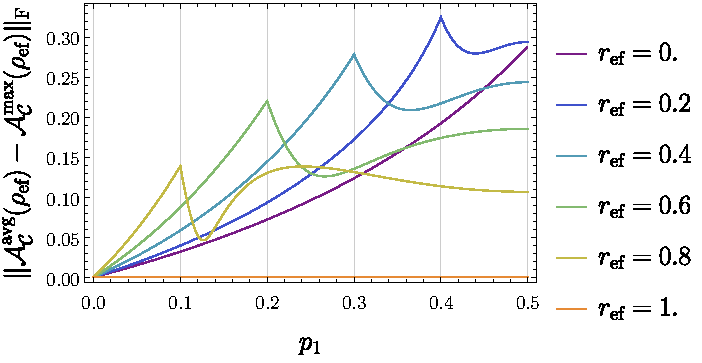
\includegraphics[width=1.\linewidth]{figures/avg_results/dist_maxent_avg_vs_p.pdf}
        \end{subfigure}%
        \begin{subfigure}{.45\textwidth}
          \centering
          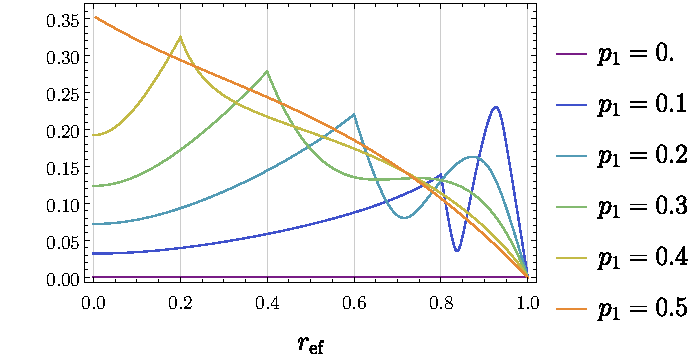
\includegraphics[width=1.\linewidth]{figures/avg_results/dist_maxent_avg_vs_z.pdf}
        \end{subfigure}
        \caption{Distancia de Frobenius entre asignaciones como función de $p_{1}$ para diferentes valores de $r_{z}$, y como función de $r_{z}$ para diferentes valores de $p_{1}$.}
    \end{figure}
\end{frame}
\begin{frame}{Discusión}
\begin{itemize}
    \item Iguales si el estado efectivo inicial es puro y si la aplicación de grano grueso se reduce a una traza parcial ($p_{1}\in\{0,1\}$).
    \item Notar que $\mcA_{\mcC}^{\max}(\Id_{2}/2)=\Id_{4}/4$ mientras que $\mcA_{\mcC}^{\avg}(\Id_{2}/2)\neq\Id_{4}/4$.
\end{itemize}
\end{frame}
%###########################
